% This file is isea.tex.  It contains the formatting instructions for and acts as a template for submissions to ISEA 2015.  It is based on the ICCC  formats and instructions.  It uses the files isea.sty, isea.bst and isea.bib, the first two of which also borrow from AAAI IJCAI formats and instructions.
% Modified from ICCC.tex by B. Bogart

\documentclass[letterpaper]{article}
\usepackage{isea}
\usepackage[pdftex]{graphicx}
\usepackage{times}
\usepackage{helvet}
\usepackage{courier}
\usepackage[numbers]{natbib}
\usepackage[normalem]{ulem}
\useunder{\uline}{\ul}{}
\pdfinfo{
/Title (Accelerating XDP Programs Using HW-based Hints)
/Author (Peter P. Waskiewicz Jr)}
% The file isea.sty is the style file for ISEA 2015 proceedings.
%
\title{Accelerating XDP Programs Using HW-based Hints}
\author{Peter P. Waskiewicz Jr. \\ Intel \\ Hillsboro, OR, USA \\ peter.waskiewicz.jr@intel.com
\And Anjali Singhai Jain \\ Intel \\ Hillsboro, OR, USA \\ anjali.singhai@intel.com
\And Neerav Parikh \\ Intel \\ Hillsboro, OR, USA \\ neerav.parikh@intel.com
\And Partha Sarangam \\ Intel \\ Hillsboro, OR, USA \\ parthasarathy.sarangam@intel.com
\newline
\newline
}
\setcounter{secnumdepth}{0}

\begin{document} 
\maketitle
\begin{abstract}
As XDP workloads continue to evolve, they are becoming more complex.  They can parse deeper into a packet to make more complex decisions, plus they may compute more complex hashing or other CPU-intensive operations to make flow-based decisions.

This talk will focus on efforts to extend the XDP framework to pass HW-based hints that have been computed by the underlying network device.  The intent is to build a framework that is vendor agnostic, so XDP programs don't need to comprehend the underlying device they're running against.

Finally, this talk will propose different directions for the changes in XDP, along with the proposed additional metadata structures.  It will also show benchmarks of certain XDP workloads with and without HW-based hints, highlighting the benefits of using these existing offloads.
\end{abstract}

\section{Keywords}

networking, kernel, ebpf, xdp, offloads

\section{Introduction}
XDP has already provided a giant leap forward in performance and efficiency for packet processing in Linux. To continue making progress, the eBPF and XDP infrastructure needs to start utilizing existing hardware offloads from a network device. This will reduce computational cycles when parsing packet headers and data, leading to more efficient eBPF and XDP programs. This progress though requires changes to the Linux kernel and surrounding eBPF infrastructure.
\newline
\newline
This paper will focus on proposed changes to eBPF and XDP for the following:
\begin{itemize}
\item Utilize HW-based offloads from a network device driver to provide hints for accelerating XDP programs
\item Share performance metrics from proof-of-concept patches highlighting the acceleration benefits of using HW hints
\item Propose future changes to the eBPF framework in LLVM, clang, and the Linux kernel, to support teaching underlying hardware which hints to provide
\item Propose additional techniques to keep XDP programs vendor-agnostic while still programming desired hints, and then consuming the hints for acceleration
\end{itemize}

\section{HW Offloaded Hints From Device Driver} 

Network hardware already computes a large number of offloads today. Future network hardware, especially with the emergence of SmartNICs \cite{smartnic2016}, will provide even more in terms of offloaded computations. Harnessing this metadata will be crucial to allow more complex eBPF and XDP programs to stay as performant as possible.
\newline
\newline
The rest of this paper discusses proposed changes to the XDP core that are built on patches from Daniel Borkman \cite{borkmann2017}, adding a metadata section to the existing {\small \texttt{xdp\_buff}} structure in the Linux kernel. Prior to these patches, an {\small \texttt{xdp\_buff}} consisted of the following:
\newline
\newline
{\scriptsize \texttt{struct xdp\_buff \{
\newline
\indent{void *data;}
\newline
\indent{void *data\_end;}
\newline
\indent{void *data\_hard\_start;}
\newline
\}
}}
\newline
\newline
After the patches, the structure now looks like this:
\newline
\newline
{\scriptsize \texttt{struct xdp\_buff \{
\newline
\indent{void *data;}
\newline
\indent{void *data\_end;}
\newline
\indent{void *data\_hard\_start;}
\newline
\indent{void *data\_meta;}
\newline
\}
}}
\newline

\begin{figure}[h]
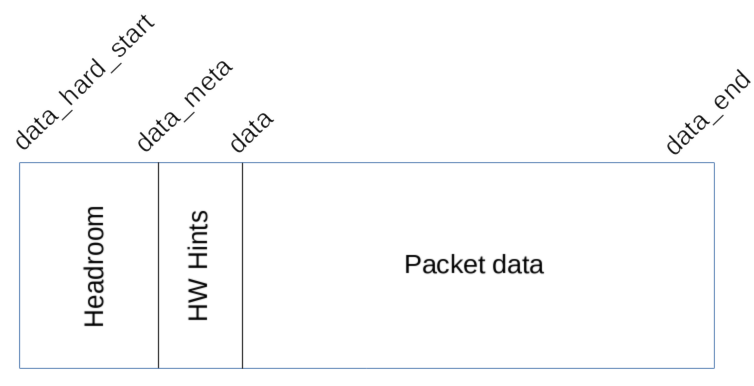
\includegraphics[width=3.31in]{xdp-metadata-layout.png}
\caption{xdp\_buff layout with metadata}
\label{xdp-metadata-layout}
\end{figure}

The new {\small \texttt{xdp\_buff}} field, {\small \texttt{"data\_meta"}}, can be used to point at opaque data sitting inside the headroom in the {\small \texttt{xdp\_buff}} memory, prior to the DMA'd packet buffer. Referring to Figure \ref{xdp-metadata-layout}, this headroom can then be parsed using proposed eBPF helper functions to extract the HW-based hints from the driver. These hints can then be used in the business logic of the XDP programs.

\subsection{Initial Performance Gains}

Initial performance gains are very promising using HW-based hints. In benchmarks with proof-of-concept patches, where hints are {\small \texttt{memcpy()}}'d from the Rx descriptor into the XDP buffer headroom, two XDP programs were used to demonstrate the gains.
\newline
\indent The system under test (SUT) was an Intel Xeon E5-2697 v2 (Ivy Bridge), using an Intel XXV710 NIC running at 25GbE. The driver on the NIC was i40e, version 2.1.14-k, with a Linux kernel version of 4.14.0-rc1+, based on a net-next snapshot with the {\small \texttt{xdp\_buff->data\_meta}} field merged.
\newline
\indent Two programs, XDP3 and XDP\_HINTS, were written to demonstrate the usage of hints. This is compared to the in-kernel XDP1 sample program, designed to parse the packet headers and then drop all traffic.  XDP3 is a copy of XDP1, however it performs no parsing at all. This is to demonstrate the smallest XDP program to take a packet and immediately drop it.  XDP\_HINTS is a modified version of XDP1, where instead of parsing packet data, it consumes metadata from the {\small \texttt{xdp\_buff}} provided by the base driver, and then drops the packet. In other words, it performs no packet parsing, but just makes decisions based off metadata.
\newline
\indent Data in Figure \ref {xdp-performance} was collected on an Ivy Bridge-class Xeon platform as the target machine. As seen in the chart, XDP1 with JIT runs at approximately 7.3 million packets/second. XDP3, with no packet parsing but with JIT, runs at approximately 22 million packets/second. XDP\_HINTS, which performs no packet parsing, but uses the HW-provided hints in the XDP metadata, also runs at 22 million packets/second. From this data with simple programs, we can see that removing the packet parsing to make a drop decision yields almost 3x in performance of XDP drop using HW-provided hints.
\newline
\indent How this metadata is expressed in the {\small \texttt{xdp\_buff}} is something the community will need to agree on moving forward. The next sections propose various approaches in how to express and consume this metadata, along with recommendations for each approach.
\begin{figure}[h]
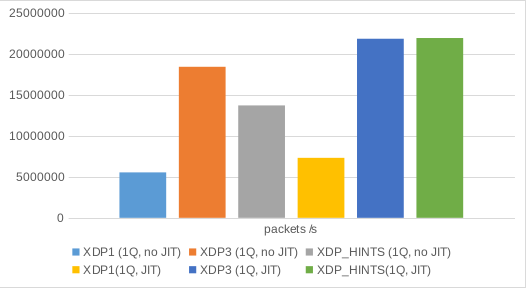
\includegraphics[width=3.31in]{xdp-programs-performance.png}
\caption{XDP With and Without HW Hints}
\label{xdp-performance}
\end{figure}

\subsection{Implementation Approach 1: Common Metadata Structure}

The most obvious approach to passing metadata through the {\small \texttt{xdp\_buff}} is to have a kernel structure that is defined to carry the data itself. This would be something each network driver would need to implement to translate HW offloads into the structure. While this would provide a vendor-agnostic solution to represent data, it imposes ABI restrictions to the XDP metadata core. Vendors would need to agree on this structure, and then this would become part of the UAPI, which means it cannot change once it is established, aside from additions. This rigidity of the interface, plus trying to have all vendors agree on a common structure to express specific hardware behaviors, is not a model believed to be sustainable moving forward.

\subsection{Implementation Approach 2: Vendor Logic in eBPF Libraries}

A different approach of processing metadata passed from a driver to the XDP core is to provide vendor-specific helper functions in the eBPF libraries in userspace. In this approach, a helper function such as {\small \texttt{bpf\_get\_hints()}} could then derive the underlying hardware, and call the vendor-specific hints-retrieval helper function. The main advantage to this approach is no kernel-level ABI is imposed through UAPI, so each vendor controls how the metadata is packed into the {\small \texttt{xdp\_buff}}. This approach can also provide a software fallback mechanism, in the case the underlying hardware doesn't provide the requested hints.
\newline
\indent However, the disadvantage to this approach is it requires eBPF and XDP programs to have knowledge of the underlying hardware they're running on. This introduces a requirement on XDP and eBPF that hasn't existed previously, where the program models avoided knowing or relying on specific hardware to operate.

\subsection{Implementation Approach 3: Chained XDP Programs With Helper Functions}

Another approach to process metadata from the driver to the XDP core is to chain multiple XDP programs together. The first XDP program would be attached either to the whole device driver, or to a specific Rx queue (see section \textit{Express Hints via eBPF Sections}). As seen in Figure \ref{xdp-chained-programs}, this initial XDP program would have the device-specific knowledge to translate the metadata passed through the XDP headroom from the driver. Acting as a shim program, it would then call the larger XDP program where the business logic resides. However, the larger XDP program would not require any device-specific knowledge, and would use new eBPF helper functions to extract the processed metadata from the first XDP program.

\begin{figure}[h]
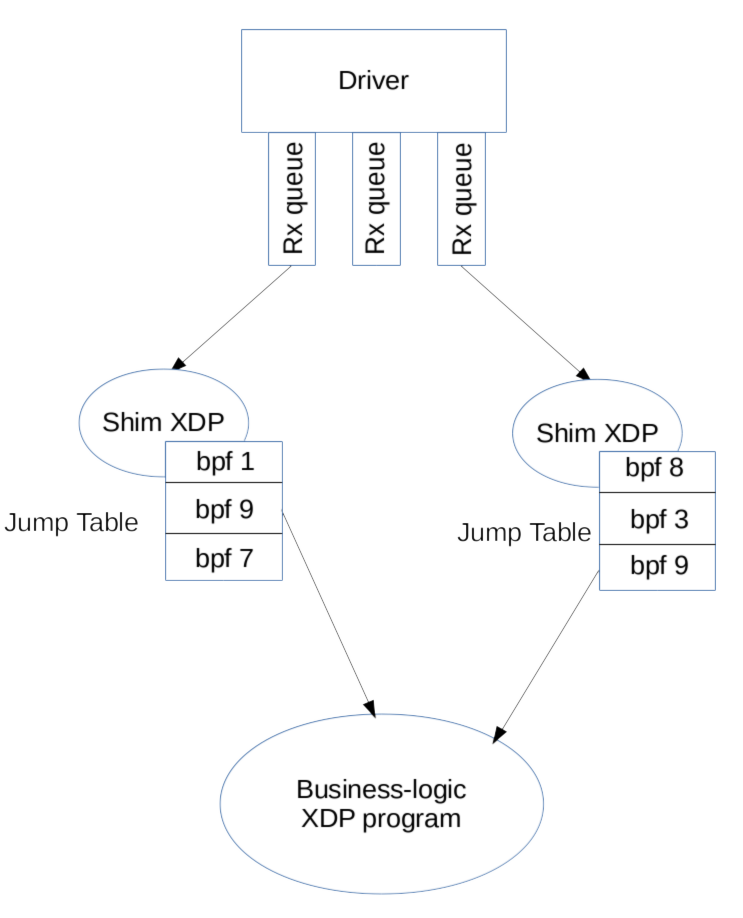
\includegraphics[width=3.31in]{xdp-chained-programs.png}
\caption{Chained XDP Programs}
\label{xdp-chained-programs}
\end{figure}

\indent This approach is still under investigation as a viable solution as of the writing of this paper. Open items needing design are:
\begin{itemize}
\item The dynamic updating of a jump table if a user wishes to update the business-logic XDP program downstream of the shim XDP program
\item Defining what all of the helpers would be (e.g. {\small \texttt{bpf\_get\_rxhash()}}, {\small \texttt{bfp\_get\_ptype()}}, etc.)
\item Defining how the data from the shim XDP progam would be presented to the downstream XDP program
\item Measure the performance impact of chaining programs together for XDP, versus running all in one contained eBPF program
\end{itemize}
As these items are developed and tested, our intent is to provide these patches for RFC to the upstream community.

\section{Dynamic Programming of HW Hints}

As SmartNICs become more available and flexible, having a robust and flexible mechanism to program them is crucial. Today, some offloads and flow match actions can be programmed using \textit{tc} and/or \textit{devlink}. However, these mechanisms currently do not have queue-level granularity to program a flow, nor do they currently have mechanisms to attach an eBPF program to consume the HW hints being requested. While the support for this can be added to these existing tools over time as SmartNICs continue to mature, we believe that also expressing the HW hints that would be most useful to XDP and broader eBPF programs should be expressed as part of the eBPF program itself.

\subsection{Using tc}

The \textit{tc} framework has had hardware-offload support added over the past few years. These mechanisms can be expressed via \textit{tc-flower} for known fields in a flow, or \textit{tc-u32} for unnamed offsets within a flow. These can be utilized to program an underlying Rx pipeline in hardware to match fields in flows, and then provide the HW hints that can be utilized by the attached eBPF/XDP programs. However, there are two areas requiring investigation to provide the flexibility that will be needed to fully utilize the SmartNICs.
\newline
\indent A SmartNIC may have the flexibility to aggregate Rx queues into groups, or even into single queues, with various offloads. Consider Receive-Side Scaling (RSS), where one may wish to have separate RSS domains for different queue groups, based on different match criteria. For example, if one flow is a tunneled 6-in-4 flow (IPv6 inside IPv4), one may wish to match that flow signature in hardware, and direct it to a specific set of RSS queues for further offloading/hashing. However, if another flow is identified as a non-tunneled IPv6 flow, one may wish to match that flow signature in a different set of RSS queues for further processing. In order to utilize \textit{tc} for this level of granularity, the framework will need to comprehend how to program a single queue in the Rx pipeline, or a set of queues in that same pipeline, while programming the match criteria within \textit{tc-flower} or \textit{tc-u32}. This capability does not exist today in the current \textit{tc} framework.
\newline
\indent As SmartNICs evolve over time, new match criteria with new hints or new actions to take on filter hits will be added to devices. For \textit{tc} to comprehend these new hints and/or actions, kernel changes will be required to add support for these new hints and actions. This will cause adoption of new hints and actions with SmartNIC updates to be delayed in the field, which may not be desirable to end users and customers wanting to fully utilize their SmartNICs. A more dynamic solution not requiring kernel changes may be desirable.
\newline
\indent The next step past programming the underlying Rx pipeline to generate match criteria and resulting metadata is how to utilize it within an attached eBPF/XDP program. While programming the Rx pipeline can help manage the offloads and flow segragation across the Rx queues, the provided metadata needs to be expressed in such a way that the underlying XDP programs can understand and parse. Since this mechanism of programming the Rx pipeline using \textit{tc} is completely separate and disjoint from the actual eBPF programs running against the device, coordination between these two layers may be very difficult. In addition, when the XDP core and framework is evolved to utilize an XDP program per-Rx queue, programming this Rx pipeline per-queue, or per-queue group, can become quite messy to coordinate with which XDP program will be running on which queues. This issue of coordination is dealt with using an alternate approach in the next section.

\subsection{Express Hints via eBPF Sections}

An alternate approach this paper proposes for programming the Rx pipeline for HW-based hint extraction is to express the desired hints via new eBPF program sections. These would be part of the eBPF program itself that is loading against a device, queue group, or queue, and would provide the necessary information to a device driver to program the pipelines. This would also have the direct benefit that the eBPF program that is programming the Rx pipeline has direct knowledge of which HW-based hints should be coming across from the underlying driver.
\newline
\indent A goal of this approach should also be to keep this interface as vendor-agnostic as possible. In other words, the hints themselves could start with a known base set of desirable hints (more on this below), allowing an eBPF program to load on any hardware. This would provide the ability for software to still compute a hint that is needed for the eBPF/XDP program's execution, but the underlying hardware isn't capable of providing that specific hint. This would be a software-fallback mode. This part of the proposal is still in its infancy as of the writing of this paper.
\newline
\indent Another approach to keep the business logic of the eBPF program vendor-agnostic, while providing the pipeline programming via eBPF, is to utilize the previously described HW-hints implementation proposal, \textit{Chained XDP Programs With Helper Functions}. This approach would allow any hardware-specific logic potentially required for Rx pipeline programming to be contained in the shim XDP program, and then that program would also know exactly which hints to extract and send to the business-logic XDP program.
\newline
\newline
The following examples are proposals of what the new eBPF sections would look like:
\newline
\newline
\textbf{\underline{Example 1: RSS hash definition and extraction:}}
\newline
\newline
{\scriptsize \texttt{struct bpf\_hw\_hints\_def SEC("hw\_hints") rx\_hash = \{
\newline
\indent .type = RSS\_HASH,
\newline
\indent .size = sizeof(\_\_u32),
\newline
\indent /* It may be a good idea to also specify in some form
\newline
\indent \space * the fields that should be used for computing
\newline
\indent \space * the hash.
\newline
\indent \space * Example: Inner-most L3 src addr and L4 src port
\newline
\indent \space */
\newline
\indent .fields = \{ INNER\_L3\_SRC, INNER\_L4\_SRC\},
\newline
\indent .mask = \{0x00ffff, 0xffff\},
\newline
\indent .key = \{xyz123\},
\newline
\};
}}
\newline
\newline
\textbf{\underline{Example 2: Packet-type identification and extraction:}}
\newline
\newline
{\scriptsize \texttt{/* PTYPE values should be agreed upon between the
\newline
\space \space * SW and the HW providing the hints. The driver
\newline
\space \space * may have to do the translation between the two.
\newline
\space \space */
\newline
struct bpf\_hw\_hints\_def SEC("hw\_hints") rx\_ptype = \{
\newline
\indent .type = PTYPE,
\newline
\indent .size = sizeof(\_\_u16),
\newline
\};
}}
\newline
\newline
\textbf{\underline{Example 3: Packet match resulting in action or map offload:}}
\newline
\newline
{\scriptsize \texttt{struct bpf\_hw\_hints\_def SEC("hw\_hints") rx\_match = \{
\newline
\indent .type = PACKET\_MATCH,
\newline
\indent .fields = \{PTYPE, INNER\_L3\_SRC, INNER\_L4\_SRC\},
\newline
\indent .mask = \{0xff, 0.0.ff.ff, 0xffff\},
\newline
\indent .value = \{0x10, 10.10.20.2, 65\},
\newline
\indent /* This hint adds a match rule into HW, which creates a
\newline
\indent \space * SW-defined result when HW finds a match
\newline
\indent \space */
\newline
\indent .result = 25,
\newline
\indent .size = sizeof(\_\_u32),
\newline
\};
}}
\newline
\newline
\indent Figure \ref{xdp-hint-types} is a table of proposed well-known hints to program and utilize in eBPF programs to consider.

\begin{figure}[h]
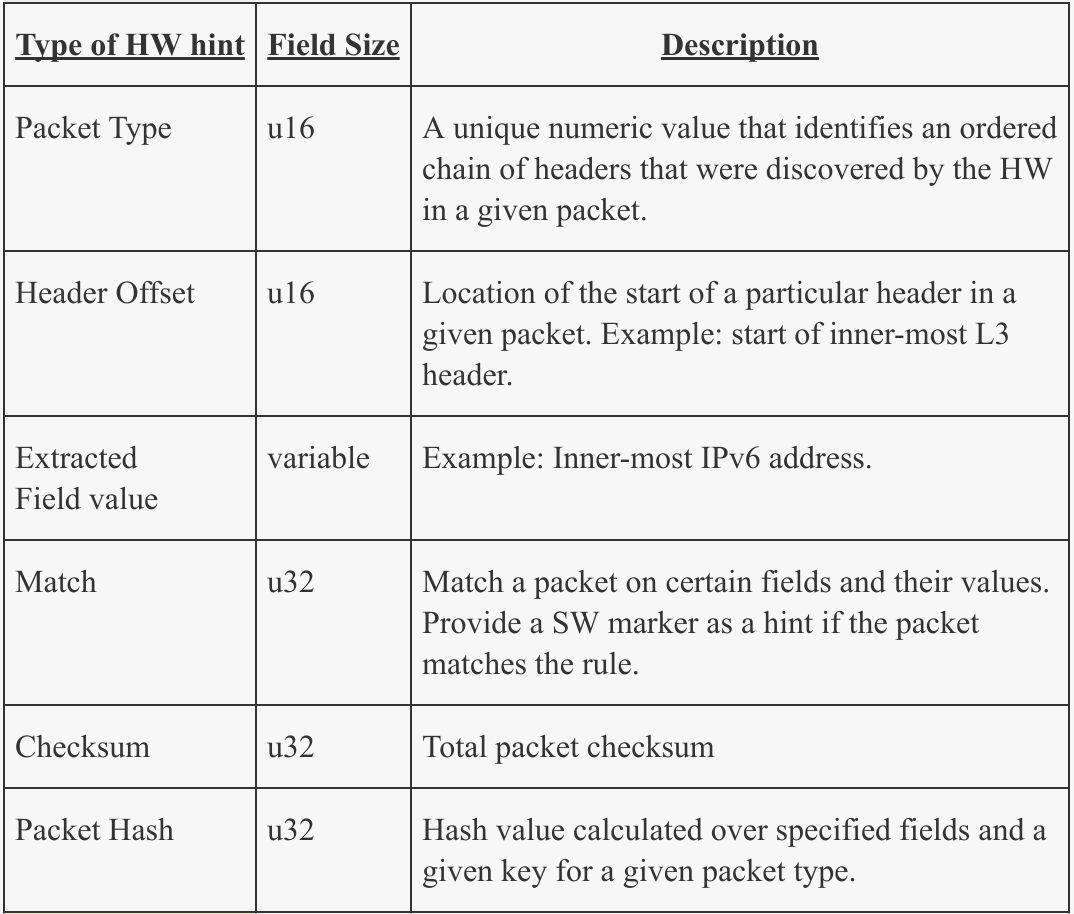
\includegraphics[width=3.31in]{xdp-hint-types.png}
\caption{Proposed HW-Based Hints}
\label{xdp-hint-types}
\end{figure}

\indent In order for this eBPF-based Rx pipeline programming to work, it would need to touch the entire eBPF toolchain. LLVM/clang would need to know how to lay out the new ELF sections, and then the kernel verifier and loader would need to understand how to pull these ELF sections out of the main program. A new .ndo\_ops field may need to be added for the eBPF loader to call a network driver to load the Rx pipeline sections, however this is still under discussion as of the writing of this paper. Once the basic concepts are agreed upon for the general direction, RFC patches will be provided to the Linux Netdev community.

\section{Conclusion}
As XDP programs become more and more complex with packet processing and parsing, the natural direction is to utilize as many offloads to maximize efficiency and performance. And with network hardware becoming smarter and more flexible, these offloads and their programmability will fit the needs of XDP's evolution towards this goal. However, the expression of the hints from hardware, and programming of the underlying hardware to present the hints, is something the Linux kernel network community will need to work together on to best design a sustainable and scalable model.

\section{Acknowledgments}
We would like to acknowledge the NetDev 2.2 selection committee for inviting us to submit and present this paper.

\bibliographystyle{pj-netdev-2.2}
\bibliography{pj-netdev-2.2}

\section{Author Biographies}
Peter Waskiewicz Jr (PJ) is a Senior Linux Kernel Engineer in the Networking Division of Intel's Communications Group. He has maintained and helped create the igb, ixgbe, and i40e wired Ethernet network drivers, the initial Tx multiqueue support in the Linux kernel network stack, and added Data Center Bridging support to the Linux kernel. He also worked in Intel's Open Source Technology Center on the x86 kernel tree, enabling advanced features in the Broadwell and Skylake microarchitectures. Prior to returning to Intel, PJ was a Principal Engineer at NetApp in the SolidFire division, where he was the chief Linux kernel and networking architect for the SolidFire scale-out cloud storage platform.
\newline
\newline
Anjali Singhai Jain is a Software Architect at Intel's Networking Division. Having worked exclusively in Networking for the past 13 years at Intel, she has seen and contributed towards many generations of Network software Architecture, software implementation, and design of Network Hardware devices. Currently she focuses her work at Intel in defining next-generation silicon features and software programming models.
\newline
\newline
Neerav Parikh is a Software Architect with Intel's Connectivity Group focusing on Ethernet Networking Software. He has worked on Intel's ixgbe and i40e Linux device drivers, focusing on features related to FCoE, DCB, and QoS. Prior to joining Intel, Neerav worked as a Technical Architect enabling SAS/SATA/FC-based Storage software products.
\newline
\newline
Partha Sarangam is a Senior Principal Engineer at Intel. He has been the lead SW Product Architect for most of the major Ethernet Controllers Intel has brought to the market in the last decade. Currently, Partha is the Chief SW Architect for Intel's future Ethernet Controllers. Partha has extensive SW development experience ranging from application software to device driver development.

\end{document}
